\documentclass{../presentation}

\usepackage{../Tsinghua}

\title{基于深度学习的推荐算法研究}

\author{姚欣培\;皇甫硕龙}

\setstretch{1.2}

\begin{document}
    \begin{frame}
        \maketitle
    \end{frame}

    \small

    \section{Problem Definition \& Data}

    \begin{frame}
        \frametitle{Problem Definition}

        Build a recommendation model based on Amazon review data to introduce new items to customers.

        \textbf{Dataset} 5-core Amazon product data \cite{ni2019justifying}. Field are identical to the dataset given in class.
    \end{frame}

    \section{Local Attention \& GRU \cite{zhu2021deep}}

    \subsection{Introduction}
    \begin{frame}
        \frametitle{Introduction}

        \begin{itemize}
            \item Background
            \begin{itemize}
                \item Information Overload $\rightarrow$ Recommendation system(CF, MF)
            \end{itemize}
            \item Disadvantage of CF
            \begin{itemize}
                \item Items with less rates have little chance to be recommended
                \item Do not take supplementary information into consideration
                \item Data sparsity and the cold start problem
            \end{itemize}
        \end{itemize}

    \end{frame}

    \begin{frame}
        \frametitle{Introduction}

        \begin{itemize}
            \item Recommendation algorithm based deep learning
            \begin{itemize}
                \item DNN
                \item CNN\cite{kim2014convolution, ji2019twitter} - text classification, emotion analysis, neural language model and information processing
                \item RNN(LSTM, GRU) - widely used especially in extracting sequence features
            \end{itemize}
            \item Problem
            \begin{itemize}
                \item Only considered the weight of a certain review
                \item Less taking consideration of words' or phrases' weights and sequence information between them in a review
            \end{itemize}
        \end{itemize}

    \end{frame}

    \subsection{Model and Result}
    \begin{frame}
        \frametitle{Model Construction}

        \begin{columns}
            \begin{column}{0.3\linewidth}
                \begin{figure}
                    \centering
                    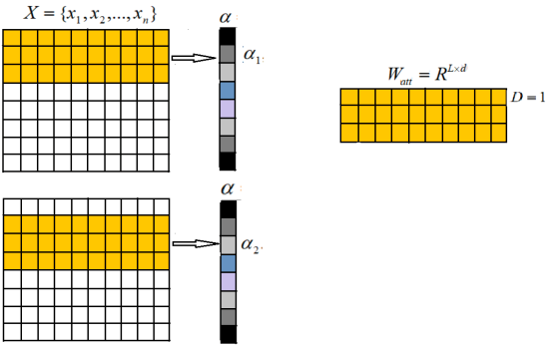
\includegraphics[width=5cm]{img/gp01-1.png}
                \end{figure}
            \end{column}
            \begin{column}{0.6\linewidth}
                \begin{enumerate}
                    \item Users' review processing
                    \begin{itemize}
                        \small
                        \item One-hot encoding words: embedding word vector into $d$ dimension
                    \end{itemize}
                    \item Local Attention Mechanism
                    \begin{itemize}
                        \item Central word $x_i$ with window size $D$
                        \item $\alpha_i=\sigma\left(x_i^{att}\otimes W_{att}+b_{att}\right)$, where $x_i^{att}$ is the context of $x_i$
                    \end{itemize}
                    \item Convolutional Neural Network Module
                    \begin{itemize}
                        \item $z_i^{(l−att)}=\max\left\{\text{ReLU}(X^{att}\ast W_l+b_{l-att})\right\}$
                    \end{itemize}
                \end{enumerate}
            \end{column}
        \end{columns}

    \end{frame}

    \begin{frame}
        \frametitle{Model Construction}

        \begin{columns}
            \begin{column}{0.4\textwidth}
                \begin{figure}
                    \centering
                    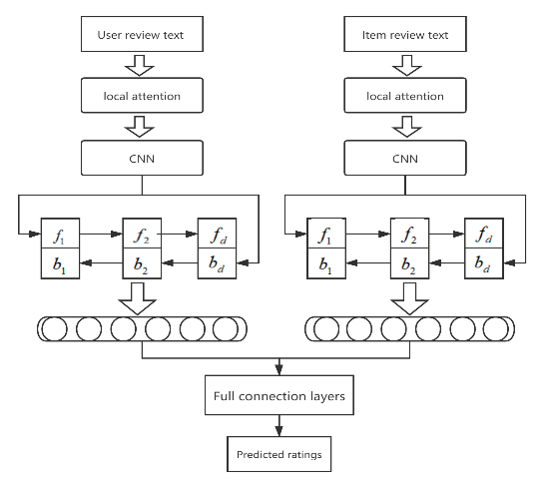
\includegraphics[width=5cm]{img/gp01-2.png}
                \end{figure}
            \end{column}

            \begin{column}{0.5\textwidth}
                \begin{enumerate}
                    \setcounter{enumi}{3}
                    \item Bidirectional Gated Recurrent Unit
                    \begin{itemize}
                        \item $u_f=\text{GRU}_{\text{forward}}\left(z^{(l-att)}\right)$
                        \item $u_b=\text{GRU}_{\text{backward}}\left(z^{(l-att)}\right)$
                        \item $p_u=u_f\oplus u_b$
                    \end{itemize}
                    \item Full Connection Layers
                    \begin{itemize}
                        \item $\hat r_{ui}=W_{mul}(p_u\cdot q_u)+b_u+b_i+\mu$
                    \end{itemize}
                \end{enumerate}

                \begin{equation}
                    J=\frac{1}{N}\sum_{u, i}\left(\hat r_{ui} - r_{ui}\right)^2
                \end{equation}
            \end{column}
        \end{columns}

    \end{frame}

    \subsection{Result \& Discussion}

    \begin{frame}
        \frametitle{Result}

        \begin{figure}
            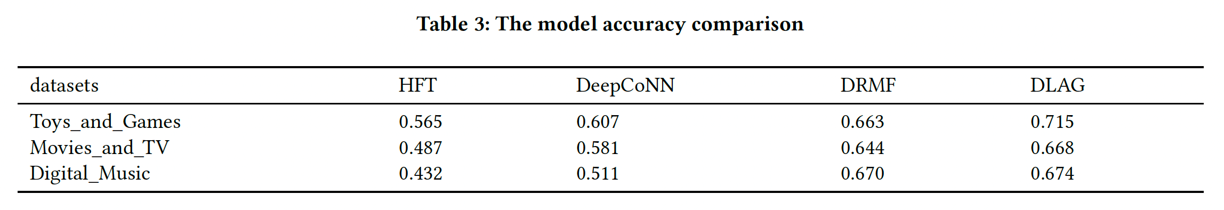
\includegraphics[width=0.7\linewidth]{img/gp01-3.png}
            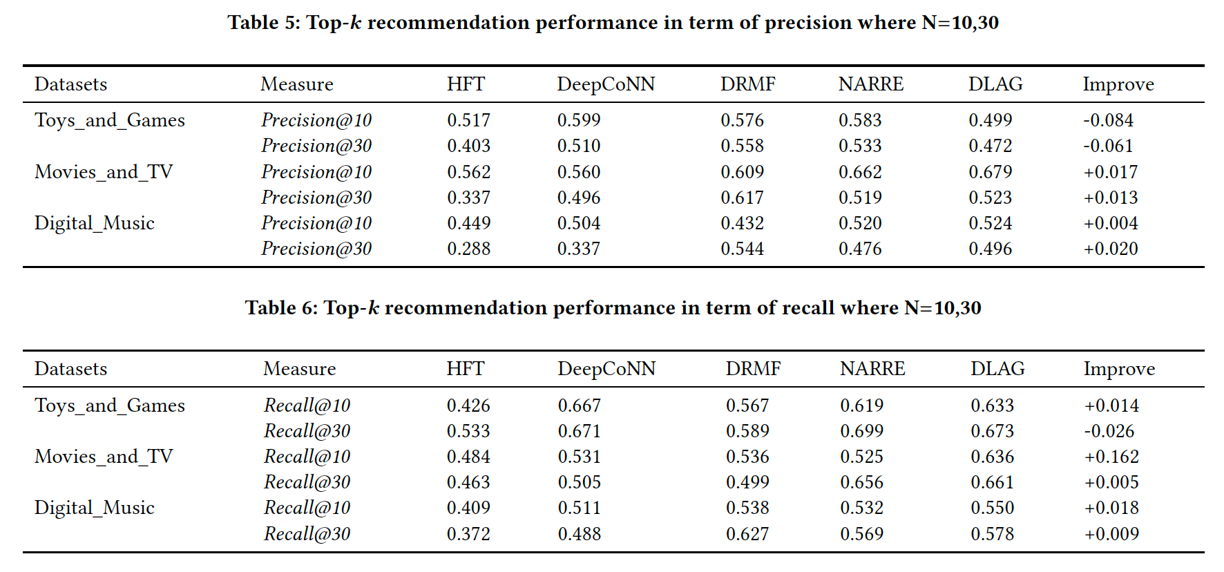
\includegraphics[width=0.7\linewidth]{img/gp01-4.png}
        \end{figure}

    \end{frame}

    \begin{frame}
        \frametitle{Discussion}

        \begin{itemize}
            \item Contribution
            \begin{enumerate}
                \item Propose a method to improve recommendation algorithm, which could extract users' and items' attributes with review data;
                \item Take the context of words in reviews into consideration;
                \item Using attention mechanism to find the key words of items and users;
                \item Excellent performance compared with other baselines;
            \end{enumerate}
            \item Drawback
            \begin{enumerate}
                \item Do not take time varying factor into consideration;
                \item Without emotional analysis of reviews to confirm the users' preference;
            \end{enumerate}
        \end{itemize}

    \end{frame}

    \section{Deep Reinforcement Learning \cite{liu2022redrl}}

    \subsection{Introduction}
    \begin{frame}
        \frametitle{Introduction}

        From "recommendation system" to "interactive recommendation system".

        \begin{itemize}
            \item IRS is more flexible, optimize for users' long-term utility, which can be formalized as a Markov Decision Process
            \item RL can efficiently optimize the decision process of IRS
        \end{itemize}

        Problems:

        \begin{enumerate}
            \item Data sparsity problem is present for most IRSs.
            \item When action space is large, making decisions is difficult.
        \end{enumerate}

        Solution: use review data to enhance the IRS model

    \end{frame}

    \begin{frame}
        \frametitle{Markov Decision Process}

        MDP $(\mathcal S, \mathcal A, \mathcal P, \mathcal R, \gamma)$ - Optimal policy $\pi: \mathcal S\rightarrow \mathcal P(\mathcal A)$

        \begin{enumerate}
            \item $\mathcal S$: state space. $s_t \in \mathcal S$ indicates user's preference at $t$, from items $c_t = \{i_1, i_2, \cdots, i_n\}$ which \textbf{positively} interacts with.
            \item $\mathcal A$: action space. $a_t \in \mathcal A$ indicates users' choice at $t$.
            \item $\mathcal R$: reward. Mapping $r: \mathcal S\times \mathcal A\rightarrow \mathcal R$, represents a user's feedback (utility) to a given item.
            \item $\mathcal P$: transition probability. Given a set of items $s_t$ indicates a user previously interacted with at time $t$, and item $i$ which was recommended at time $t$.
            \begin{equation}
                s_{t+1} = \begin{cases}
                    s_t & \text{declined} \\
                    s_t \cup \{i\} & \text{accepted}
                \end{cases}
            \end{equation}
            \item $\gamma$: discount factor. Balances long-term rewards and immediate rewards.
        \end{enumerate}

    \end{frame}

    \subsection{Model Construction}
    \begin{frame}
        \frametitle{Model Construction}

        \begin{columns}
            \begin{column}{0.4\linewidth}
                \begin{figure}
                    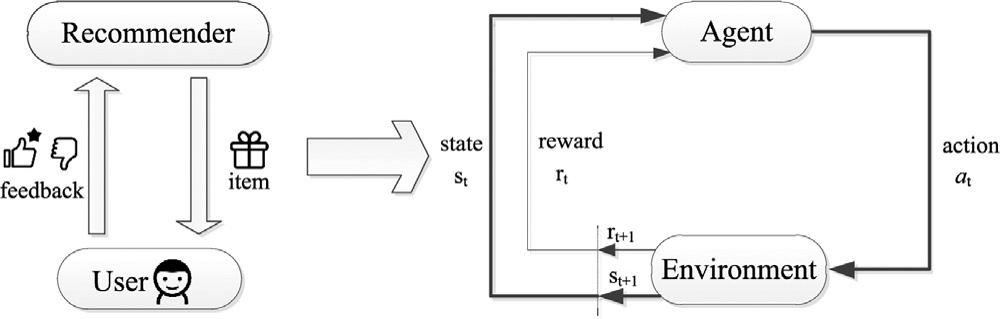
\includegraphics[width=\linewidth]{img/gp01-5.jpg}
                \end{figure}
            \end{column}
            \begin{column}{0.55\linewidth}
                \begin{figure}
                    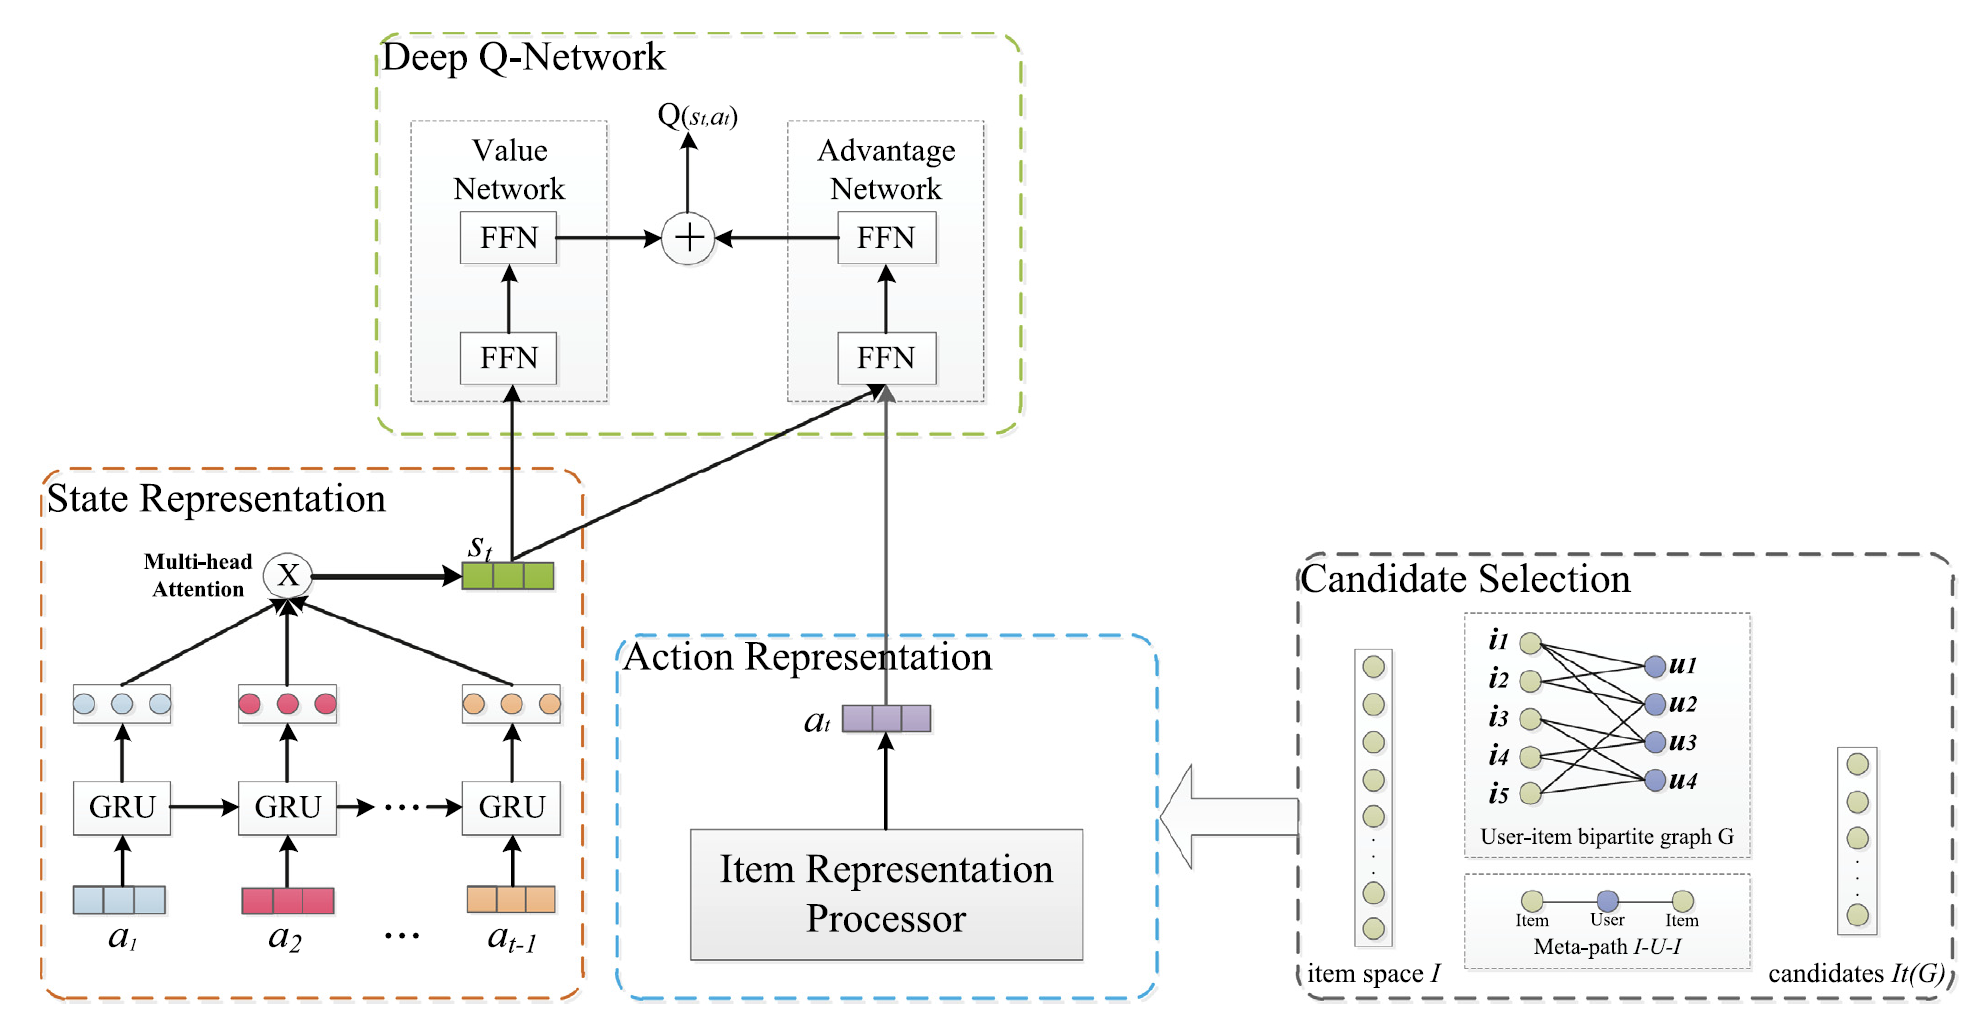
\includegraphics[width=\linewidth]{img/gp01-6.png}
                \end{figure}
            \end{column}
        \end{columns}

        \begin{columns}
            \begin{column}{0.5\linewidth}
                \begin{itemize}
                    \item Action representation: review enhanced
                    \item State representation: attention enhanced
                \end{itemize}
            \end{column}
            \begin{column}{0.5\linewidth}
                \begin{itemize}
                    \item Candidate selection: meta path-guided
                    \item Deep Q-network based policy learning
                \end{itemize}
            \end{column}
        \end{columns}

    \end{frame}

    \subsection{Result \& Discussion}

    \begin{frame}
        \frametitle{Result}

        \begin{columns}
            \begin{column}{0.5\linewidth}
                \begin{figure}
                    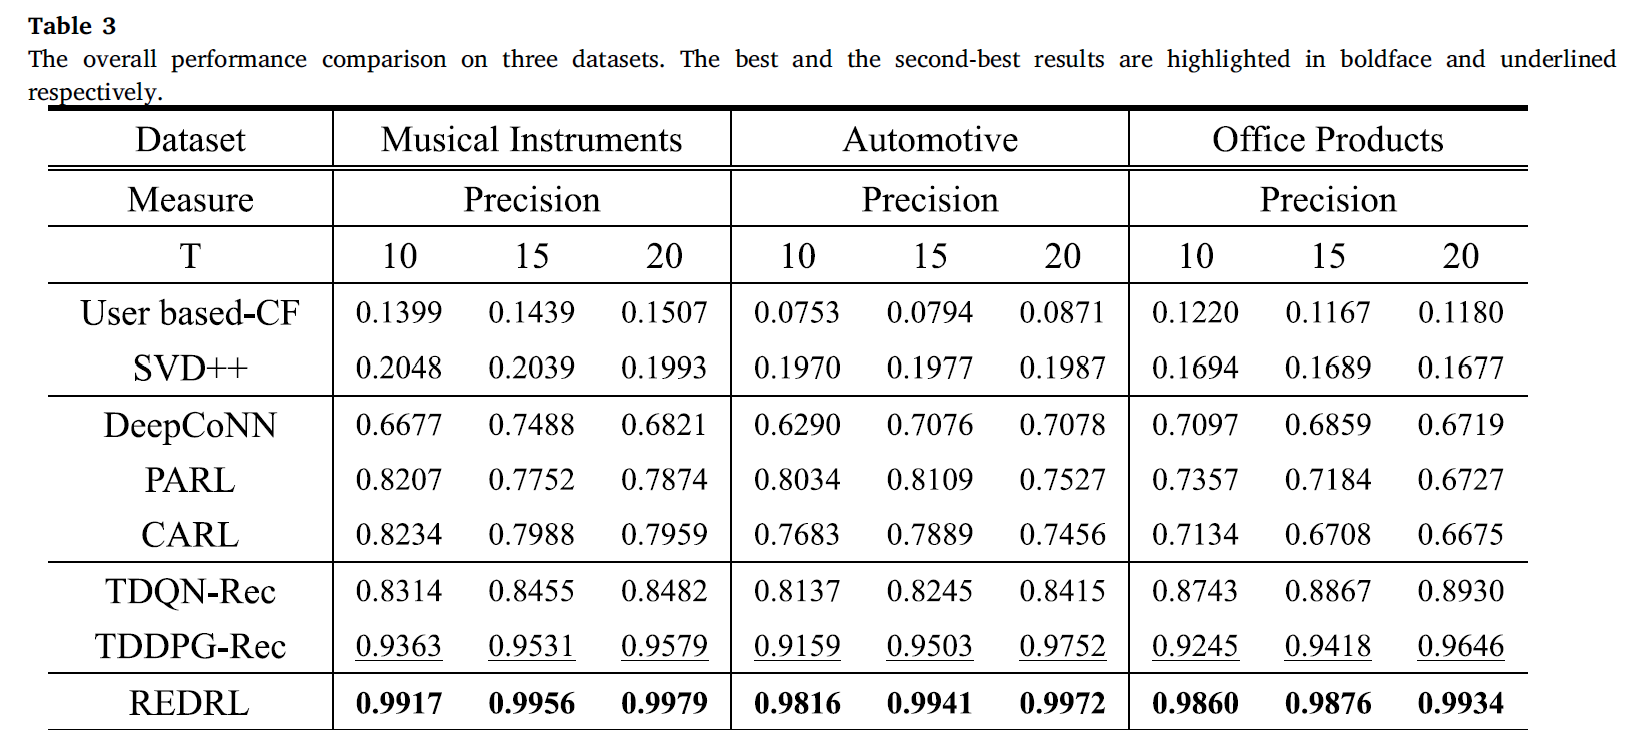
\includegraphics[width=\linewidth]{img/gp01-7.png}
                \end{figure}
            \end{column}
            \begin{column}{0.5\linewidth}
                \begin{figure}
                    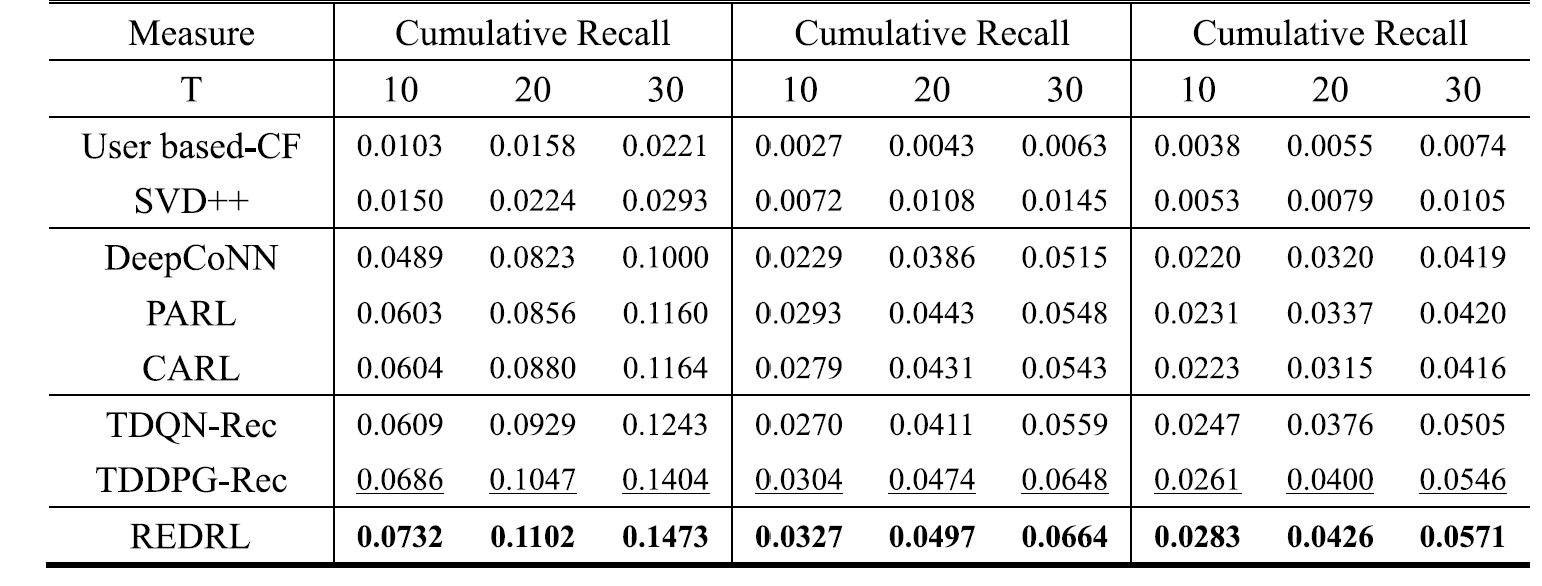
\includegraphics[width=\linewidth]{img/gp01-8.png}
                \end{figure}
            \end{column}
        \end{columns}
        \vspace*{0.25cm}
        More: sensitivity of parameters and model variants
    \end{frame}

    \begin{frame}
        \frametitle{Discussion}

        Model long-term dynamic preferences of users accurately and discriminately for comprehensive interactive recommendation.

        \begin{itemize}
            \item Formalization: MDP
            \item Model: DRL
            \begin{itemize}
                \item Semantic structure information
                \item Meta-paths in heterogeneous information networks
                \item Multi-head self-attention technique
            \end{itemize}
        \end{itemize}

        Future work: apply a more advanced model to the current model.

    \end{frame}

    \section{References}
    \begin{frame}[allowframebreaks]
        \frametitle{Reference}
        \footnotesize
        \bibliographystyle{plain}
        \bibliography{gp01}
    \end{frame}
\end{document}